\section{Simulation Setup}

\begin{figure}[H]
	\centering
	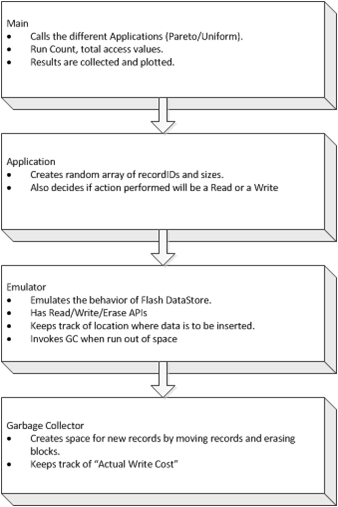
\includegraphics[width=0.4\textwidth]{C:/Ananth/OSU/CETI/MS-Thesis/MS-thesis-Report/imgs/Simulation-Flow-chart.png}
	\captionof{figure}{Simulator Flow chart} \label{Simulator-FlowChart}
\end{figure}

As shown in figure~\ref{Simulator-FlowChart}, {\bf Main} program controls the number of times the simulation is to be run and which application gets called among other things. It also collects the results returned by the {\bf Application} and generates the graphs. It invokes the {\bf Application} program which contains the implementation for Uniform, Pareto or BiModal type of distributions. Based on the toss of a coin, it decides if the next operation will be a read or a write. Every read and write operation invokes the {\bf Emulator} which contains functionalities such as reading/writing a record, maintaining the indices of the records within the Flash and so on. When space runs out, the {\bf Emulator} invokes the {\bf Garbage Collector} whose primary purpose is to free up space by moving around active records and erasing a block of inactive records. It is successful if it finds sufficient space for the next record to be inserted and it returns an exception back to the Emulator if it is not able to find space in the entire Flash.


%\subsection{Functions used in Simulator}
%
%\begin{center}
%\begin{tabular}{ |c| p{5cm} | }
%	\hline
%	\multicolumn{2}{ |c| } {Main} \\
%	\hline
%		\multicolumn{2}{ |c| }{\textit{runAppUniformDistribution}} \\
%	\hline
%		\multirow{1}{*} {\textbf{Parameter}} & \textbf{Description} \\ \hline
%		appRunCount & Application run count \\
%		appRunCount & Application run count \\
%
%		\hline
%		\multirow{1}{*} {\textbf{Return Value}} & \textbf{Description} \\ \hline
%		appRunCount & Application run count \\
%		appRunCount & Application run count \\
%	\hline
%\end{tabular}
%\end{center}
%%
%\qquad
%%
%\begin{center}
%\begin{tabular}{ |c| p{5cm} | }
%	\hline
%	\multicolumn{2}{ |c| } {Application} \\
%	\hline
%		\multicolumn{2}{ |c| }{\textit{AppUniformDistribution}} \\
%	\hline
%		\multirow{1}{*}{\textbf{Parameter}} & \textbf{Description} \\ \hline
%		seedVal & Application run count \\
%		seedVal & Application run count \\
%
%		\hline
%		\multirow{1}{*}{\textbf{Return Value}} & \textbf{Description} \\ \hline
%		seedVal & Application run count \\
%		seedVal & Application run count \\
%	\hline
%\end{tabular}
%\end{center}
%%
%\qquad
%%
%\begin{center}
%\begin{tabular}{ |c| p{5cm} | }
%	\hline
%	\multicolumn{2}{ |c| } {Emulator} \\
%	\hline
%		\multicolumn{2}{ |c| }{\textit{runAppUniformDistribution}} \\
%	\hline
%		\multirow{1}{*}{\textbf{Parameter}} & \textbf{Description} \\ \hline
%		appRunCount & Application run count \\
%		seedVal & Application run count \\
%
%		\hline
%		\multirow{1}{*}{\textbf{Return Value}} & \textbf{Description} \\ \hline
%		seedVal & Application run count \\
%		seedVal & Application run count \\
%	\hline
%\end{tabular}
%\end{center}
%%
%\qquad
%%
%\begin{center}
%\begin{tabular}{ |c| p{5cm} | }
%	\hline
%	\multicolumn{2}{ |c| } {Garbage Collector} \\
%	\hline
%		\multicolumn{2}{ |c| }{\textit{runAppUniformDistribution}} \\
%	\hline
%		\multirow{1}{*}{\textbf{Parameter}} & \textbf{Description} \\ \hline
%		appRunCount & Application run count \\
%		seedVal & Application run count \\
%
%		\hline
%		\multirow{1}{*}{\textbf{Return Value}} & \textbf{Description} \\ \hline
%		seedVal & Application run count \\
%		seedVal & Application run count \\
%	\hline
%\end{tabular}
%\end{center}

%-----------------------------------------------------------------------------------

\section{Related Work}
\subsection{An Age-Threshold Algorithm for Garbage Collection in Log-Structured Arrays and File Systems}
	This paper compares the Greedy and Cost-Benefit algorithm with their algorithm called "Age-Threshold algorithm". Greedy considers those segments for Garbage Collection that has the least amount of active records or in other words can yield the maximum amount of space. Cost-Benefit considers those segments that will yield the maximum space but at the same time, are above a certain age. Age-Threshold considers those segments that are above a threshold. Age is determined by means of a clock. When data is moved from one segment to another by GC, the age of the new segment is the old + 1. But when a segment is erased and then new data is written, the age starts from 0. 

\subsection{Cleaning Policies in Mobile Computers Using Flash Memory}
	This paper compares the Greedy, Cost-Benefit with their algorithm - CAT (Cost Age Time). CAT algorithm claims to reduce the number of erase operations performed on a block while evenly wearing out the flash at the same time. It considers the age of the data, the cleaning cost and the number of times a segment has been erased. A segment is chosen such that the formula $CleaningCost * 1/Age * Count of cleaning$ is minimized. It also considers different ways of redistributing data (within the same block and across several blocks). The algorithm is compared for data patterns such as those with varying localities of reference, uniform access and so on.

	Grouping data across segments based on their hotness degree is similar to generational algorithms. There are algorithms on opposite ends of the spectrum. One one end there are algorithms that claim longer the age of a block, the more likely to have inactive data. The other end of spectrum, algorithms claim that longer the data is not accessed, higher they can be moved to generations.

In generational, the problem is that there is a large amount of hot data that is being marked as cold. Very soon after the data is moved to a higher generation, data tends to get inactivated. This results in wasted move cost. Most of the inefficiency comes from thinking of hot data as cold (move hot data too soon). For Uniform, FIFE is the best, but for Pareto age definitely has to be considered. 

\subsection{Questions}
	What is the recommended algorithm for Pareto distribution? 
	Are any of the generational algorithms good or should they not be used?

%-----------------------------------------------------------------------------------
\subsection*{Conclusions and Future Work}
	Flash devices are making a great headway in becoming the storage device of choice in Mobile and Embedded systems. But they still have disadvantages such as a slow write speed which prevent them from being used as the primary storage device replacing RAMs. In order for them to perform optimally, Garbage Collectors are very important. This work analyzed the performance of five different GC algorithms against the most common of the traffic patterns in real-world applications (Uniform, Pareto and BiModal). The results that have come out of this study have gone against the existing results in current literature and hence have the potential to make rapid progress towards using Flash as primary storage. 

%-----------------------------------------------------------------------------------
\subsection*{Future work}
	

%-----------------------------------------------------------------------------------
\subsection*{Acknowledgements}
	I am grateful to Dr.Mukundan Sridharan who guided me during the course of this work. Thanks also to Dr.Rajiv Ramnath who during our weekly meetings, guided me in the right direction by asking lot of questions and helping me get the answers for them. My sincere gratitude also to Dr.Kenneth Parker and Dr.Anish Arora for giving me the opportunity to work on this wonderful project. Last but not the least, I am thankful to the professors and friends who helped me when I was stuck at a difficult problem. 